\documentclass[12pt]{article}

% Packages
% page size
\usepackage{geometry}
\geometry{a4paper, left=25mm, right=25mm, top=25mm, bottom=25mm}

% bibliography management
\usepackage[backend=biber, style=authoryear, sorting=ynt]{biblatex}
\addbibresource{biblio_st_conv_diff_1d.bib}

% math
\usepackage{amsmath}

% figures
\usepackage{graphicx}
\graphicspath{ {F:/myApps/projects/cfd/cfd-codes/st-conv-diff-1d/analysis/} }

% better figure captions (scriptsize, footnotesize, small, normalsize, large, Large)
\usepackage[font=normalsize, labelfont=bf]{caption}

% cross-referencing !!! usually must be imported at the end
\usepackage{hyperref}
\hypersetup{
    colorlinks=true,
    linkcolor=blue,
    filecolor=magenta,      
    urlcolor=cyan,
    % pdfpagemode=FullScreen,
    pdftitle={CFD 01},
    pdfauthor={Alts},
    % pdfstartpage={2},
}
% \urlstyle{same}


% Info
\title{CFD Project n+01: Solution of one-dimensional convection-diffusion equation}
\author{A. Tsvetkov}
\date{Last updated \today}


\begin{document}


\begin{titlepage}

\maketitle{}

\begin{abstract}
In this project, a numerical solution of a one-dimensional convection-diffusion equation was developed and programmed in the C programming language. The finite-difference disretisation approach was used. The results of the upwind-differencing (UDS) and central-differencing (CDS) schemes were compared on uniform and non-uniform meshes of different sizes. It was demonstrated that the UDS remains bounded irrespective of the mesh coarseness but exhibits high numerical diffusion. On the other hand, the CDS requires a local Peclet number of less than 2 to avoid oscillations, but agrees very well with the exact solution when the condition is satisfied. Both schemes showed optimal results when used on a non-uniform mesh, which has fewer nodes in regions of a low gradient and more nodes in regions with a high gradient.
\end{abstract}

\thispagestyle{empty}

\end{titlepage}


\newpage
\pagenumbering{roman}
\tableofcontents


\newpage
\pagenumbering{arabic}
\section{Introduction}
\label{sec:intro}

This project is a part of an ongoing effort to develop new skills and competencies in CFD and to present them in the form of a portfolio of projects. The current project aims to develop a complete numerical solution of a stationary convection-diffusion equation in one dimension using the C programming language. The following objectives have been identified.

\begin{itemize}
\item A discretisation of the governing equation using the finite-difference approach.
\item An implementation of the numerical solution in a computer program written in the C programming language.
\item An analysis of results, including an investigation of the role of the Peclet number on the accuracy of the final solution.
\end{itemize}

The project largely follows a worked example in \textcite{FerzigerCFD}, chapter 3.10. It was noted that the problem describes a flow when convection is balanced by stream-wise diffusion, which is not representative of the majority of real-life flows. Typically, convection is balanced by a pressure gradient or a diffusion in a cross-stream direction. Therefore, the authors warn that conclusions drawn from solving this problem might not be directly applicable to actual flows. Nevertheless, the project holds some learning value and illustrates a few noteworthy issues.

A short disclaimer. While the project attempts to highlight author's competencies (or lack thereof), it is not intended to be fully comprehensive. Some aspects are omitted and/or are not explored in great detail, intentionally or otherwise, in favour of progressing the project quicker and moving on to other projects, because there is a lot to learn.


\section{Governing equations}
\label{sec:govEq}

The finite difference discretisation involves covering a solution domain by a grid of nodes, approximating a partial differential equation with nodal values of the variables, writing down a corresponding algebraic equation, and finally solving algebraic equations for all nodes as a system. According to \textcite{FerzigerCFD}, the method is simple, effective, and lends itself for higher-order schemes. However, it appears to be primarily used with structured grids, which limits its applicability to simple geometries only. Another disadvantage of the method is that it does not enforce conservation by default.

The starting point for the finite difference distretisation method is a partial differential equation. For the current problem of one-dimensional stationary convection-diffusion, it takes the following form \parencite{FerzigerCFD}.

\begin{equation}
    \frac{\partial (\rho u \phi)}{\partial x} = \frac{\partial}{\partial x} \left( \Gamma \frac{\partial \phi}{\delta x} \right)
\end{equation}

\noindent where $\rho$, $\phi$, and $\Gamma$ are the fluid density, the transported quantity, and the diffusion coefficient respectively.

The intended result of the discretisation process is a system of linear algebraic equations. Each node is expected to have one equation of the form

\begin{equation}
    A_{i-1} \phi_{i-1} + A_{i} \phi_{i} + A_{i+1} \phi_{i+1} = S_{i}
\end{equation}

\noindent where $A_{i}$, $\phi_{i}$, and $S_{i}$ are the coefficients, the values of the transported quantity at corresponding nodes, and source terms respectively.

Next, the generation of mesh is discussed followed by the discretisation of the convective and diffusive terms.


\subsection{Mesh}
\label{sec:mesh}

Coordinates of the mesh nodes can be calculated using the formula

\begin{equation}
    x_i = x_{left} + \frac{x_{right} - x_{left}}{\sum_{m = 0}^{n - 1} r^m} \sum_{k = 0}^{i} r^k
\end{equation}

\noindent where $x_i$ is the i-th point coordinate, $x_{left}$ is the left boundary coordinate, $x_{right}$ is the right boundary coordinate, $n$ is the number of points, and $r$ is the refinement factor.


\subsection{Convective term}
\label{sec:convection}


\paragraph{Central differencing scheme (CDS)}

For the purposes of this project, noteworthy properties of the CDS are

\begin{itemize}
    \item conditional boundedness at $Pe < 2$ (this is a sufficient but not necessary condition), and
    \item second-order accuracy.
\end{itemize}

Question. What about conservativeness, transportiveness (\textcite{VerMalCFD}, ch. 5.4)?

The CDS can be implemented using the following relations.

\begin{subequations}

\begin{equation}
    \left. \frac{\partial (\rho u \phi)}{\partial x} \right|_{i} \approx \rho_i u_i \frac{\phi_{i+1} - \phi_{i-1}}{x_{i+1} - x_{i-1}}
\end{equation}

\begin{equation}
    A_{i-1} = - \frac{\rho_i u_i}{x_{i+1} - x_{i-1}}
\end{equation}

\begin{equation}
    A_{i+1} = \frac{\rho_i u_i}{x_{i+1} - x_{i-1}}
\end{equation}

\end{subequations}

While technically $A_i = 0$, it is conventional to express it as a negative sum of the previous two coefficients, which, in this case, cancel each other out.

\begin{equation}
    A_{i} = - \left( A_{i-1} + A_{i+1} \right)
\end{equation}


\paragraph{Upwind differencing scheme (UDS)}

Unlike the CDS, the UDS is:

\begin{itemize}
    \item unconditionally bounded, and
    \item first-order accurate.
\end{itemize}

Question. What about conservativeness, transportiveness (\textcite{VerMalCFD}, ch. 5.4)?

The UDS can be implemented using the following relations.

\begin{subequations}

\begin{equation}
    \left. \frac{\partial (\rho u \phi)}{\partial x} \right|_{i} \approx 
    \begin{cases}
        \rho_i u_i \dfrac{\phi_{i} - \phi_{i-1}}{x_{i} - x_{i-1}} & \text{if $u > 0$} \\
        \rho_i u_i \dfrac{\phi_{i+1} - \phi_{i}}{x_{i+1} - x_{i}} & \text{if $u < 0$}
    \end{cases}
\end{equation}

\begin{equation}
    A_{i-1} = \frac{min(- \rho u_i, 0)}{x_{i} - x_{i-1}}
\end{equation}

\begin{equation}
    A_{i+1} = - \frac{min(\rho u_i, 0)}{x_{i+1} - x_{i}}
\end{equation}

\end{subequations}

\subsection{Diffusive term}
\label{sec:diffusion}

The diffusive term is approximated using the CDS for both outer and inner derivatives. Note that, initially, the inner derivative is approximated using the points midway between nodes. Then, the second approximation utilises the nodal values.

\begin{subequations}

\begin{multline}
    \left. \frac{\partial}{\partial x} \left(\Gamma \frac{\partial \phi}{\delta x}\right) \right|_i \approx
    \frac{\left(\Gamma \frac{\partial \phi}{\partial x}\right)_{i+0.5} - \left(\Gamma \frac{\partial \phi}{\partial x}\right)_{i-0.5}}{0.5 \left(x_{i+1} - x_{i-1}\right)} \approx
    \frac{\Gamma \frac{\phi_{i+1} - \phi_{i}}{x_{i+1} - x_{i}} - \Gamma \frac{\phi_{i} - \phi_{i-1}}{x_{i} - x_{i-1}}}{0.5 \left(x_{i+1} - x_{i-1}\right)} \approx \\
    \frac{2 \Gamma}{\left(x_{i+1} - x_{i-1}\right) \left(x_{i+1} - x_{i}\right)} \left(\phi_{i+1} - \phi_{i}\right) -
    \frac{2 \Gamma}{\left(x_{i+1} - x_{i-1}\right) \left(x_{i+1} - x_{i-1}\right)} \left(\phi_{i} - \phi_{i-1}\right)
\end{multline}

\begin{equation}
    A_{i-1} = \frac{- 2 \Gamma}{\left(x_{i+1} - x_{i-1}\right) \left(x_{i+1} - x_{i}\right)}
\end{equation}

\begin{equation}
    A_{i+1} = \frac{- 2 \Gamma}{\left(x_{i+1} - x_{i-1}\right) \left(x_{i+1} - x_{i-1}\right)}
\end{equation}

\end{subequations}


\subsection{Solution of algebraic equations}
\label{sec:solution}

The equations are assembled in matrices and solved using the Tri-Diagonal Matrix (Thomas) Algorithm. The method is essentially a Gauss elimination algorithm, but further streamlined to take advantage of the tri-diagonal nature of the solved matrices. The method is not iterative in its simplest implementation, when the matrix is indeed tri-diagonal. While it is possible to extend the method to more-than-three-diagonal matrices by making it iterative, it does not appear to be used much in commercial codes. Nevertheless, it was a good learning experience to code the TDMA.


\section{Implementation}
\label{sec:implementaion}

This section briefly discusses some implementation details of the outlined numerical solution.


\subsection{Program structure}
\label{sec:progStructure}

The implementation consists of two programs, a `mesher' and a `solver'. The mesher handles mesh generation, while the solver computes the solution. This task division decouples the two steps and resembles how it is done in real CFD software (probably).


\subsubsection{Mesher}
\label{sec:mesher}

The mesher accepts settings from the \verb|meshSettings.txt| file, generates the mesh based on the settings, and writes the points to the \verb|meshPoints.txt| file for a later use by the solver. 

For this project, the mesh can be controlled by 

\begin{itemize}
\item a start and an end coordinates (in one dimension);
\item a number of points;
\item a refinement factor $r$, where $r > 1$ means that the distance between points gradually increases from left to right, while $r < 1$ clusters points closer to the start coordinate. 
\end{itemize}


\subsubsection{Solver}
\label{sec:solver}

The solver contains the bulk of the code. The functionality is divided into the following blocks.

\begin{description}
\item[read\_mesh()] reads the mesh file and stores it in a global variable;
\item[read\_settings()] reads settings and stores them in a global struct-variable. The settings include information such as initial values, boundary values, and scheme selection;
\item[initialise()] allocates memory for the necessary arrays (e.g. matrices of coefficients, sources, solutions) and initialises them with the initial values;
\item[contruct\_matrices()] constructs matrices based on the provided parameters and schemes and computes the coefficients of the discretised equations;
\item[solve\_tdma()] solves the system with the TDMA method;
\item[write\_results()] writes the results for a later post-processing;
\item[free\_mem()] frees the memory, only affects dynamically-allocated global variables.
\end{description}

While the bulk of the mentioned functions handles input-output and error checking (with an exception of the \verb|solve_tdma()| function), perhaps the most theory-related snippets of the code can be found in the \verb|A_e()| and \verb|A_w()| functions, which compute the dicretisation coefficients as outlined in section \ref{sec:govEq}.


\subsection{Code assessment}
\label{sec:assessment}

The following aspects of the code might pose problems and are worth improving in later programs.

\begin{description}

\item[Better functions for reading settings] Right now, the input files are required to have a rigid structure (certain order and names for entries). In the code, every required entry has its own \verb|fgets| and/or \verb|sscanf/fscanf| statement. It would be more convenient and scalable to have some sort of a loop that goes through an entire file, records key-value pairs, and then compares it against a dictionary with all required fields to check if everything is supplied.

\item[Scheme selection] Checking for the scheme name happens for every coefficient. It would be a better design if that happened only once (or a set number times instead of O(n) times).

* Revised this part by adding a conversion of \verb|scheme_name| to \verb|scheme_int| during the reading of the settings file. Subsequently, the switch operator is used to pick required coefficients.

\item[Storage and access of the A-matrix values] They are stored in a full n*n-matrix, which is wasteful because the matrix is sparse and has values on the three central diagonals only. Furthermore, in the \verb|construct_matrices()| function, a conversion of a ``1d'' index (from 0 to \verb|n_pts|) to an equivalent ``2d'' index has to take place because the matrix A, while being a 2d-matrix, is stored as a 1d-array of length \verb|n_pts**2|. It was a half-baked idea to do it like that, and I honestly don't even know what I was thinking when I was implementing it.

\item[Matrix indexing in loops] There were some questionable choices made, to put it mildly. The problem is that not all matrices have the same (or proportional) dimensions (see the previous problem). As a results, within a loop it was necessary to track positions in structurally different matrices, hence the need for two indexes, viz. \verb|i| and \verb|i_mtrx|.

\item[Other] Better organisation of files (make all utilities callable from the case root folder).

It might be prudent to store the length of arrays and matrices together with the actual values. Maybe a struct can do that.

\end{description}


\section{Results}
\label{sec:results}

Conveniently, an analytical solution exists for the problem of one-dimensional convection-diffusion. It takes the following form \parencite{FerzigerCFD}.

\begin{equation}
    \phi = \phi_0 + \frac{e^{xPe/L} - 1}{e^{Pe} - 1} \left( \phi_L - \phi_0 \right)
    \label{eq:exactSol}
\end{equation}

\begin{equation}
    Pe = \frac{\rho u L}{\Gamma}
    \label{eq:Pe}
\end{equation}

The following parameters were used for the numerical solution: $x_{left} = 0$, $x_{right} = 1$, $rho = 1$, $\Gamma = 0.02$.

Figure \ref{fig:first} shows a comparison between the exact solution, the solution using the CDS scheme, and the solution using the UDS scheme. Both numerical solutions were obtained on a uniform mesh with 11 nodes.

\begin{figure}
    \centering
    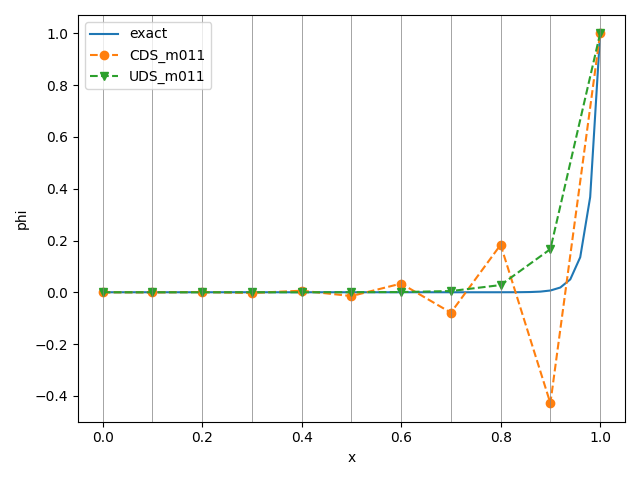
\includegraphics[width=1.0\textwidth]{results_m011}
    \caption{first}
    \label{fig:first}
\end{figure}

Evidently, the CD scheme produces an oscillating result. This can be explained by the high local Pe number of 5, which can be calculated by substituting the distance between nodes $dx = 0.1$ into eq. \eqref{eq:Pe}. The UDSscheme, while remains bounded on the coarse mesh, is not very accurate and leads to high numerical diffusion.

Next, results are obtained for a uniform mesh with 51 nodes, which gives $Pe = 1$. The results are illustrated in figure \ref{fig:second}. With the Peclet number being below 2, the threshold for boundedness of the CDS, the field distribution appears to follow the analytical solution closely. As for the UDS, while its accuracy appears to have increased, it still produces larger diffusion.

\begin{figure}
    \centering
    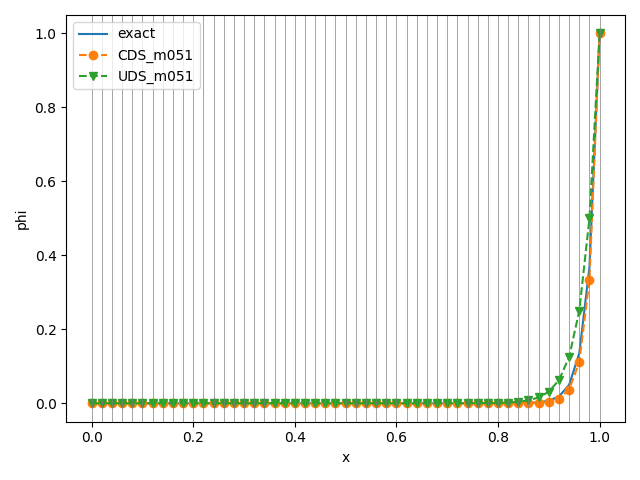
\includegraphics[width=1.0\textwidth]{results_m051}
    \caption{second}
    \label{fig:second}
\end{figure}

The final set of results is obtained for a non-uniform mesh with 11 nodes and a refinement factor $r = 0.7$, which gives larger nodes on the left and smaller nodes on the right, where the gradient is the steepest. Figure \ref{fig:third} highlights that this node arrangement produces results similar to the mesh with 51 uniformly-spaced nodes but at the same computational cost as the mesh with 11 uniformly-spaced nodes.

\begin{figure}
    \centering
    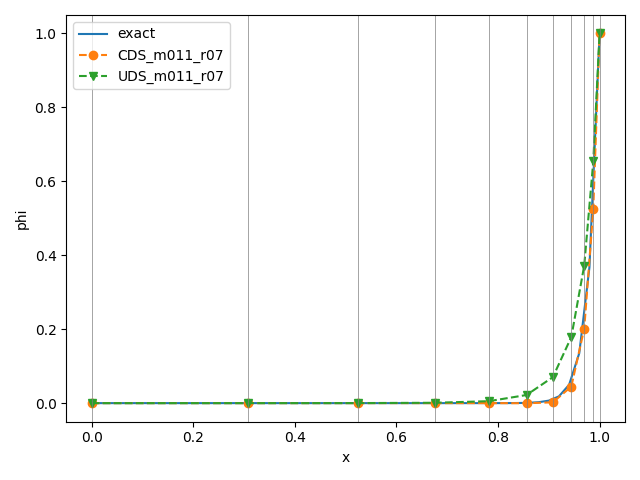
\includegraphics[width=1.0\textwidth]{results_m011_r07}
    \caption{third}
    \label{fig:third}
\end{figure}

Interestingly, after a closer look at the numerical results of the CD scheme on 11 non-uniformly-spaced nodes (see table \ref{tab:my-table}), the solution still oscillates, albeit with a much smaller amplitude. This behavior is expected as the Pe number exceeds 2 in 6 out of 10 nodes.

\begin{table}
    \centering
    \caption{Table}
    \label{tab:my-table}
    \begin{tabular}{ccccc}
    \textbf{xi} & \textbf{Pe} & \textbf{CDS} & \textbf{$>/<$} & \textbf{exact} \\
    \hline
    0.00 &  0.00 &  0.00e+00 & $>$ & 0.00e+00 \\
    0.31 & 15.44 & -2.70e-05 & $<$ & 9.75e-16 \\
    0.52 & 10.81 &  1.00e-05 & $>$ & 4.81e-11 \\
    0.68 &  7.56 & -5.00e-05 & $<$ & 9.26e-08 \\
    0.78 &  5.29 &  7.20e-05 & $>$ & 1.84e-05 \\
    0.86 &  3.71 & -2.92e-04 & $<$ & 7.51e-04 \\
    0.91 &  2.59 &  2.15e-03 & $<$ & 1.01e-02 \\
    0.94 &  1.82 &  4.49e-02 & $<$ & 6.18e-02 \\
    0.97 &  1.27 &  2.02e-01 & $<$ & 2.20e-01 \\
    0.99 &  0.89 &  5.25e-01 & $<$ & 5.36e-01 \\
    1.00 &  0.62 &  1.00e+00 & $>$ & 1.00e+00
    \end{tabular}
\end{table}

Perhaps a conclusion that should be drawn from this set of results is that it is more important to sufficiently resolve the regions of flow where variables change steeply, rather than to chase satisfaction of strict theoretical criteria. As long as sufficient accuracy for a problem at hand is achieved, some unboundedness here and there is acceptable, especially if it has benefits such as decreased computational costs.

This conclusion, however, raises a few questions, such as

\begin{itemize}
    \item How to judge accuracy when a point of comparison does not exist?
    \item What is ``sufficient'' accuracy for a given application?
    \item If the sufficient accuracy and the function gradient are connected, can this link be numerically quantified?
\end{itemize}

Answering these questions falls outside the scope of this project, and they are left as is for now.


\section{Conclusions}
\label{sec:conclusions}

In this project, the numerical solution of the 1D convection-diffusion equation was developed and programmed in the C programming language. The finite-difference discretisation approach was used. The results of the UD and CD schemes were compared on uniform and non-uniform meshes of different sizes. It was demonstrated that the UDS remains bounded irrespective of the mesh coarseness but exhibits high numerical diffusion. On the other hand, the CDS requires a local Pe number of less than 2 to avoid oscillations, but agrees very well with the exact solution when the condition is satisfied. Both schemes showed optimal results when used on a non-uniform mesh, which has fewer nodes in regions of low gradient and more nodes in regions with a high gradient. This mesh appears to strike a balance between accuracy and computational costs.

Positive takeaway points from the project:

\begin{itemize}
    \item the program works correctly;
    \item using C was pretty fun.
\end{itemize}

Negative takeaway points from the project, that should be improved (see section \ref{sec:assessment} for details):

\begin{itemize}
    \item storing the matrix of coefficients should have been done in a more memory-efficient way;
    \item indexing the matrices was wonky;
    \item reading settings files should be more flexible;
    \item better familiarity with the language is advised.
\end{itemize}

Neutral takeaway points from the project:

\begin{itemize}
    \item the theory behind the solution was somewhat straightforward;
    \item the implementation of the solution was slightly less straightforward.
\end{itemize}


\printbibliography[heading=bibintoc, title={Bibliography}]


\end{document}
